\documentclass[11pt,a4paper]{article}
\usepackage[utf8]{inputenc}
\usepackage[vietnamese]{babel}
\usepackage{amsmath,amssymb}
\usepackage[version=4]{mhchem}
\usepackage{geometry}
\geometry{top=1.5cm,bottom=1.2cm,left=1.4cm,right=1.4cm,headheight=28pt,headsep=12pt,footskip=18pt}
\usepackage{graphicx}
\usepackage{xcolor}
\usepackage{tabularx}
\usepackage{array}
\usepackage{tikz}
\usepackage{fancyhdr}
\usepackage{enumitem}
\usepackage{multido}
\usepackage{tcolorbox}
\usepackage{colortbl}

\definecolor{hfRed}{HTML}{D32F2F}
\definecolor{hfGreen}{HTML}{8BC390}
\definecolor{mainGreen}{HTML}{2E7D32}
\definecolor{solBlue}{HTML}{1565C0}
\definecolor{tableGreen}{HTML}{E8F5E9}

\usepackage{ex_test}

\pagestyle{fancy}
\fancyhf{}
\renewcommand{\headrulewidth}{0.75pt}
\renewcommand{\headrule}{\hbox to\headwidth{\color{hfGreen}\leaders\hrule height \headrulewidth\hfill}}
\renewcommand{\footrulewidth}{0.75pt}
\renewcommand{\footrule}{\hbox to\headwidth{\color{hfGreen}\leaders\hrule height \footrulewidth\hfill}}

\fancyhead[L]{\small\itshape\color{hfRed}Tài liệu lưu hành nội bộ}
\fancyhead[R]{\small\color{hfRed}Thầy \textbf{TRẦN VĂN THẠNH} - 0777.470.803}

\fancyfoot[L]{\footnotesize\itshape\color{hfRed}CS1: 6/15 Nguyễn Hoàng, P. Kim Long, TP Huế \quad|\quad CS2: 24 Đặng Thái Thân, TP Huế}
\fancyfoot[R]{\small\textbf{\color{hfRed}Trang \thepage}}

\setlength{\parindent}{0pt}
\setlength{\parskip}{2pt}

\begin{document}

\begin{minipage}[t]{0.48\textwidth}
\textbf{TRƯỜNG THPT NGUYỄN HUỆ}\\
\textbf{TỔ LÝ – HOÁ – CN}\\
\textit{ĐỀ CHÍNH THỨC}\\
\textit{(Đề thi có 04 trang)}
\end{minipage}
\hfill
\begin{minipage}[t]{0.48\textwidth}
\raggedleft
\textbf{\color{hfRed}KIỂM TRA GIỮA KỲ I – NĂM HỌC 2026 – 2027}\\
\textbf{Môn: HOÁ HỌC, Lớp 11}\\
\textit{Thời gian: 45 phút (không kể thời gian phát đề)}\\
\textbf{MÃ ĐỀ: 1204}
\end{minipage}

\vspace{4pt}
\noindent
\textit{Họ và tên thí sinh:} \dotfill \textit{Lớp:} \dotfill \textit{SBD:} \dotfill

\vspace{2pt}
\noindent
\textit{\footnotesize (Cho biết nguyên tử khối: $\ce{H = 1; N = 14; O = 16; K = 39; Ca = 40}$).}

\vspace{2pt}
\hrule color{hfGreen} height 0.5pt


\vspace{4pt}
\noindent
\textbf{\large\color{hfRed}A. PHẦN TRẮC NGHIỆM (7,0 ĐIỂM)}

\vspace{2pt}
\noindent
\textbf{\large\color{mainGreen}PHẦN I. Câu trắc nghiệm nhiều phương án lựa chọn (3,0 điểm)}

\textit{Học sinh trả lời từ câu 1 đến câu 12. Mỗi câu hỏi học sinh chỉ chọn một phương án.}
\vspace{4pt}


\begin{ex}%[1204-C1]
Mưa acid là hiện tượng nước mưa có pH thấp hơn 5,6. Hai acid chủ yếu được hình thành trong khí quyển và hòa tan vào nước mưa, gây ra mưa acid là
\choice
{\ce{HCl}, \ce{HNO3}}
{\True \ce{H2SO4}, \ce{HNO3}}
{\ce{SO2}, \ce{NO_x}}
{\ce{H2SO4}, \ce{H2S}}

\end{ex}


\begin{ex}%[1204-C2]
Cho phương trình: $\ce{CO3^{2-} + H2O <=> HCO3^- + OH^-}$\\
Trong phản ứng thuận, theo thuyết Brønsted -- Lowry chất nào là base?
\choice
{\ce{HCO3^-}}
{\ce{OH^-}}
{\True \ce{CO3^{2-}}}
{\ce{H2O}}

\end{ex}


\begin{ex}%[1204-C3]
Dung dịch X có $[\ce{OH-}] = 10^{-6}\,\text{M}$. pH của dung dịch X là
\choice
{5}
{9}
{6}
{\True 8}

\end{ex}


\begin{ex}%[1204-C4]
Tại nhiệt độ không đổi, khi một phản ứng thuận nghịch đạt trạng thái cân bằng thì
\choice
{tốc độ phản ứng hoá học xảy ra chậm dần}
{\True nồng độ của các chất trong hỗn hợp phản ứng không thay đổi}
{phản ứng hoá học không xảy ra}
{nồng độ của các chất trong hỗn hợp phản ứng vẫn liên tục thay đổi}

\end{ex}


\begin{ex}%[1204-C5]
Chuẩn độ $10\,\text{mL}$ dung dịch $\ce{NaOH}$ $x\,\text{M}$ bằng dung dịch chuẩn $\ce{HCl}$ $0{,}1\,\text{M}$ với chất chỉ thị phenolphthalein như hình vẽ dưới đây:
\begin{center}
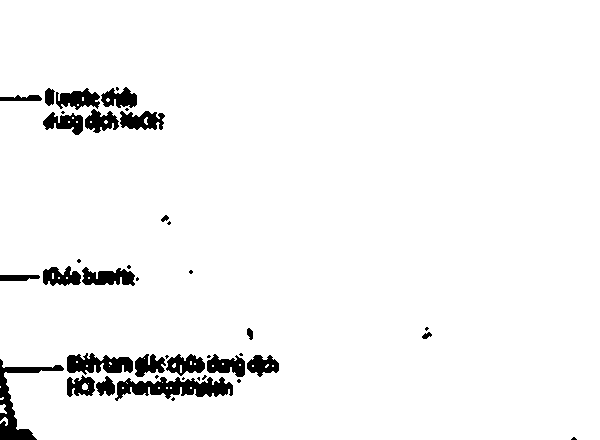
\includegraphics[width=6.0cm]{images_gk1_hoa11_ma1204/hinh_chuan_do_c5_hd.png}
\end{center}
Sau ba lần chuẩn độ, thể tích dung dịch $\ce{HCl}$ $0{,}1\,\text{M}$ đã dùng có giá trị trung bình là $15\,\text{mL}$. Giá trị của $x$ là
\choice
{\True 0,15 M}
{0,10 M}
{0,20 M}
{0,30 M}

\end{ex}


\begin{ex}%[1204-C6]
Ở trạng thái tự nhiên, nitrogen
\choice
{tự do chiếm khoảng 20\% thể tích không khí}
{\True tồn tại ở dạng đơn chất và hợp chất}
{chỉ tồn tại ở dạng đơn chất}
{chỉ tồn tại ở dạng hợp chất}

\end{ex}


\begin{ex}%[1204-C7]
Các gói bim bim được làm phồng lên bằng khí X không màu, không mùi, trơ về mặt hóa học giúp tăng thời gian bảo quản và giữ được hình dạng sản phẩm không bị vỡ vụn. X là khí nào sau đây?
\choice
{\ce{NH3}}
{\ce{O2}}
{\True \ce{N2}}
{\ce{O3}}

\end{ex}


\begin{ex}%[1204-C8]
Phản ứng nào sau đây là phản ứng thuận nghịch?
\choice
{\True $\ce{N2 + O2 <=>[t^\circ] 2NO}$}
{$\ce{C2H5OH + 3O2 ->[t^\circ] 2CO2 + 3H2O}$}
{$\ce{2KClO3 ->[t^\circ] 2KCl + 3O2}$}
{$\ce{Mg + 2HCl -> MgCl2 + H2}$}

\end{ex}


\begin{ex}%[1204-C9]
Hòa tan một ít tinh thể $\ce{CH3COONa}$ vào ống nghiệm chứa nước, có tồn tại cân bằng sau:
$$\ce{CH3COONa + H2O <=> CH3COOH + NaOH}\quad (1)$$
Thêm vài giọt phenolphthalein vào ống nghiệm thấy dung dịch chuyển sang màu hồng nhạt, tiến hành ngâm ống nghiệm trong nước nóng màu dung dịch đậm dần. Kết luận nào sau đây chính xác?
\choice
{Khi tăng nhiệt độ, cân bằng (1) chuyển dịch theo chiều nghịch}
{\True Nếu ngâm ống nghiệm trong nước đá, màu dung dịch nhạt dần}
{Chiều thuận của phản ứng (1) là quá trình tỏa nhiệt}
{Cân bằng (1) không phụ thuộc vào nhiệt độ}

\end{ex}


\begin{ex}%[1204-C10]
Phân tử ammonia được tạo thành bởi một nguyên tử nitrogen liên kết với ba nguyên tử hydrogen. Dạng hình học của phân tử ammonia là
\choice
{\True chóp tam giác}
{tứ giác}
{tam giác đều}
{vuông phẳng}

\end{ex}


\begin{ex}%[1204-C11]
Chất nào sau đây khi hòa tan vào nước không phân li ra ion ?
\choice
{\ce{CH3COOH}}
{\True \ce{C2H5OH}}
{\ce{HCl}}
{\ce{NaCl}}

\end{ex}


\begin{ex}%[1204-C12]
Trong quá trình đốt cháy nhiên liệu hóa thạch như than đá và dầu nặng, thường sản sinh các khí $\ce{NO, NO2}\dots$ Tên gọi của $\ce{NO2}$ là
\choice
{ammonia}
{\True nitrogen dioxide}
{dinitrogen oxide}
{nitrogen monoxide}

\end{ex}


\vspace{6pt}
\noindent
\textbf{\large\color{mainGreen}PHẦN II. Câu trắc nghiệm đúng sai (2,0 điểm)}

\textit{Học sinh trả lời từ câu 1 đến câu 2. Trong mỗi ý a), b), c), d) ở mỗi câu, học sinh chọn đúng hoặc sai.}
\vspace{4pt}


\begin{ex}%[1204-P2-C1]
Phương trình hóa học của phản ứng tổng hợp ammonia từ nitrogen và hydrogen bằng quá trình Haber như sau:
$$\ce{N2(g) + 3H2(g) <=>[t^\circ, p, \text{xt Fe}] 2NH3(g)}\quad \Delta_\text{r}H^\circ_{298} = -91{,}8\,\text{kJ}\quad (*)$$
\choiceTF
{\True Liên kết hoá học trong phân tử $\ce{NH3}$ là liên kết cộng hoá trị có cực}
{Do có hàm lượng nitrogen cao (82,35\% theo khối lượng) nên ammonia được sử dụng trực tiếp làm phân đạm rất hiệu quả}
{Có thể nhận biết muối ammonium bằng cách cho muối tác dụng với dung dịch kiềm thấy thoát ra chất khí làm quỳ tím ẩm hoá đỏ}
{\True Phản ứng (*) là phản ứng tỏa nhiệt. Để tăng hiệu suất tổng hợp $\ce{NH3}$ người ta cần thực hiện ở nhiệt độ thấp nhưng không quá thấp để tốc độ phản ứng không quá chậm}

\end{ex}


\begin{ex}%[1204-P2-C2]
Ở các vùng quê, người dân thường dùng phèn chua ($\ce{K2SO4.Al2(SO4)3.24H2O}$ hay $\ce{KAl(SO4)2.12H2O}$) để làm trong nước. Khi phèn chua tan vào nước thì ion $\ce{Al^{3+}}$ bị thủy phân theo phản ứng:
$$\ce{Al^{3+} + 3H2O <=> Al(OH)3 + 3H+}\quad (*)$$
\choiceTF
{\True Phèn chua là chất điện li}
{\True Dung dịch sau khi hoà tan phèn chua vào nước có $\text{pH} < 7$}
{Dung dịch phèn chua làm phenolphthalein chuyển sang màu hồng}
{Phèn chua được dùng để làm trong nước nhờ ứng dụng của phản ứng thuỷ phân ion $\ce{Al^{3+}}$. Các bụi bẩn sẽ bị cuốn theo kết tủa keo trắng $\ce{Al(OH)3}$ lắng xuống đáy nên nước sẽ trong lại. Trong phản ứng (*) $\ce{Al^{3+}}$ là base và $\ce{H2O}$ là acid}

\end{ex}


\vspace{6pt}
\noindent
\textbf{\large\color{mainGreen}PHẦN III. Câu trắc nghiệm trả lời ngắn (2,0 điểm)}

\textit{Học sinh trả lời từ câu 1 đến câu 4.}
\vspace{4pt}


\begin{ex}%[1204-P3-C1]
Trong thí nghiệm chuẩn độ dung dịch $\ce{NaOH}$ bằng dung dịch $\ce{HCl}$, người ta cho từ từ dung dịch $\ce{NaOH}$ từ burette vào bình tam giác chứa dung dịch $\ce{HCl}$ và vài giọt dung dịch phenolphthalein. Trong các dụng cụ thí nghiệm được đánh số dưới đây, burette là dụng cụ số mấy?
\begin{center}
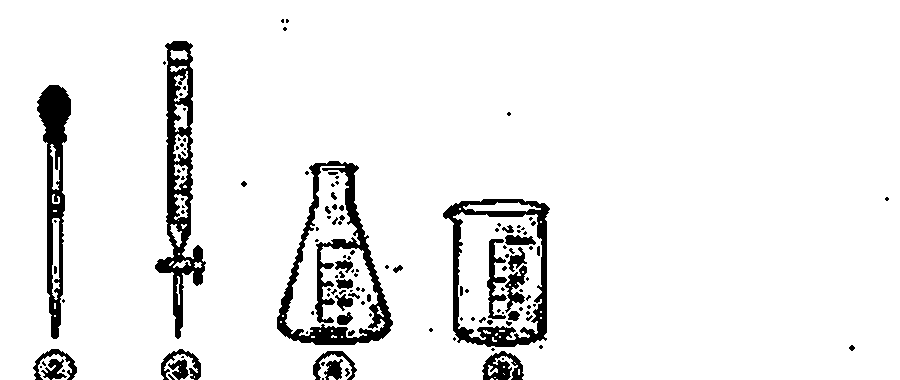
\includegraphics[width=11.5cm]{images_gk1_hoa11_ma1204/dung_cu_thi_nghiem_hd.png}
\end{center}
\textbf{Trả lời: } \dotfill

\end{ex}


\begin{ex}%[1204-P3-C2]
Cho các ứng dụng sau:
\begin{enumerate}[label=(\arabic*)]
\item Sản xuất phân đạm urea ($\ce{(NH2)2CO}$).
\item Được sử dụng làm chất làm lạnh trong thiết bị lạnh.
\item Sản xuất nitrogen.
\item Sản xuất nitric acid.
\end{enumerate}
Hãy liệt kê các ứng dụng đúng của ammonia theo thứ tự tăng dần? (Ví dụ: 123, 234...)

\textbf{Trả lời: } \dotfill

\end{ex}


\begin{ex}%[1204-P3-C3]
Cho phản ứng thuận nghịch sau ở nhiệt độ $430^\circ\text{C}$: $\ce{H2(g) + I2(g) <=> 2HI(g)}$. Nồng độ mol các chất ở thời điểm cân bằng như sau: $[\ce{H2}] = [\ce{I2}] = 0{,}107\,\text{M}$; $[\ce{HI}] = 0{,}768\,\text{M}$. Tính hằng số cân bằng $K_\text{c}$ của phản ứng ở $430^\circ\text{C}$ (làm tròn kết quả đến hàng phần mười).

\textbf{Trả lời: } \dotfill

\end{ex}


\begin{ex}%[1204-P3-C4]
Cho các phát biểu sau:
\begin{enumerate}[label=(\arabic*)]
\item Ánh sáng mặt trời bị cản trở làm ảnh hưởng đến quá trình quang hợp, gây thiếu oxygen làm cho thực vật và động vật chết.
\item Sự phân hủy xác động thực vật bởi vi khuẩn sử dụng nhiều oxygen trong nước gây nên tình trạng thiếu oxygen nghiêm trọng, làm chết cả hệ sinh thái.
\item Chất dinh dưỡng giúp thực vật và tảo sống trong nước phát triển ồ ạt.
\item Phân bón và chất dinh dưỡng bị rửa trôi xuống sông, ao, hồ.
\end{enumerate}
Hãy sắp xếp các phát biểu trên theo đúng trình tự diễn biến quá trình hình thành hiện tượng phú dưỡng thành bộ bốn số (ví dụ: 2143, 4213, ...)?

\textbf{Trả lời: } \dotfill

\end{ex}


\vspace{6pt}
\noindent
\textbf{\large\color{hfRed}B. PHẦN TỰ LUẬN (3,0 ĐIỂM)}
\vspace{4pt}


\begin{ex}%[1204-TL1]
\textbf{(1,0 điểm)} Cho cân bằng hoá học (trong bình kín) sau:
$$\ce{2NO2 (g) <=> N2O4 (g)}\quad (*)$$
\quad\quad\quad\quad\textit{(màu nâu đỏ)}\quad\quad\quad\textit{(không màu)}
\begin{enumerate}[label=\textbf{\alph*)}]
\item Cân bằng (*) chuyển dịch theo chiều nào (thuận hay nghịch) khi tăng áp suất của hỗn hợp ở điều kiện nhiệt độ không đổi? Giải thích ngắn gọn.
\item Khi hạ nhiệt độ của bình thì màu nâu đỏ nhạt dần. Phản ứng thuận là toả nhiệt hay thu nhiệt? (không giải thích).
\end{enumerate}

\noindent\textit{Bài làm:}
\multido{\i=1+1}{7}{\noindent\makebox[\linewidth]{\dotfill}\\[1.5pt]}

\end{ex}


\begin{ex}%[1204-TL2]
\textbf{(1,0 điểm)} Nước thải công nghiệp trước khi xả ra môi trường cần được thu gom và xử lý đạt tiêu chuẩn theo quy định. Theo quy chuẩn kỹ thuật quốc gia về nước thải công nghiệp, giá trị pH của nước thải công nghiệp khi xả vào nguồn tiếp nhận phải nằm trong khoảng từ 5,5 đến 9,0. Một mẫu nước thải của nhà máy X có $\text{pH} = 4$. Để đảm bảo đạt tiêu chuẩn xả thải, nhà máy sử dụng vôi sống ($\ce{CaO}$) cho vào nước thải để nâng pH từ 4 lên 7.
\begin{enumerate}[label=\textbf{\alph*)}]
\item Hãy cho biết mẫu nước thải của nhà máy X có môi trường là acid, base hay trung tính?
\item Giải thích tác dụng của vôi sống trong việc làm tăng pH của nước thải bằng phương trình hoá học?
\item Tính khối lượng vôi sống (kilogam) cần sử dụng để xử lý $6000\,\text{m}^3$ nước thải nói trên? (Bỏ qua sự thủy phân của các muối nếu có). (Không làm tròn kết quả các phép tính trung gian, chỉ làm tròn kết quả cuối cùng đến hàng phần mười).
\end{enumerate}

\noindent\textit{Bài làm:}
\multido{\i=1+1}{10}{\noindent\makebox[\linewidth]{\dotfill}\\[1.5pt]}

\end{ex}


\begin{ex}%[1204-TL3]
\textbf{(1,0 điểm)} Quá trình hình thành đạm nitrate cho đất từ nước mưa được biểu diễn theo sơ đồ sau:
$$\ce{N2 ==(1)==> NO ==(2)==> NO2 ==(3)==> HNO3 ==(4)==> H+ + NO3^-}$$
\begin{enumerate}[label=\textbf{\alph*)}]
\item Viết phương trình hóa học của các phản ứng xảy ra (ghi rõ điều kiện nếu có, mỗi mũi tên là một phản ứng hóa học).
\item Một cơn mưa rơi xuống một thửa ruộng với lượng mưa trung bình là $5\,\text{m}^3/\text{giờ}$. Hãy tính khối lượng nguyên tố nitrogen (tính bằng gam) mà thửa ruộng nhận được khi cơn mưa đó kéo dài 3 giờ? (Giả sử hàm lượng ion nitrate trong nước mưa khoảng $62\,\text{mg/L}$ và hàm lượng nitrate trong nước mưa không đổi trong suốt thời gian mưa).
\end{enumerate}

\noindent\textit{Bài làm:}
\multido{\i=1+1}{10}{\noindent\makebox[\linewidth]{\dotfill}\\[1.5pt]}

\end{ex}


\vspace{6pt}
\begin{center}
\textbf{---------- HẾT ----------}\\
\textit{\small - Thí sinh không được sử dụng tài liệu.\\
- Giám thị không giải thích gì thêm.}
\end{center}

\end{document}
